\documentclass[10pt]{exam}

\usepackage{tikz}
\usepackage{amsmath}
\usepackage[margin=0.5in]{geometry}
\usepackage{soul}

\newcommand{\ds}{\displaystyle}


\begin{document}
\pagestyle{empty}
\subsection*{Midterm 1 Review Problems \hfill Math 140}


\begin{questions}

\question Solve $\ds \frac{6}{x+5} + \frac{1}{2(x+5)}= 1$.
\begin{solution}
\end{solution}
\vfill
\hrule


\question Simplify $\ds  \frac{30 a}{5} \cdot \sqrt{\frac{b^2}{9a^6}}$
\begin{solution}
$$\frac{2b}{a^2}$$
\end{solution}
\vfill
\hrule

\question Factor to find all of the roots of $y= x^3-x^2-12x$, and then use the axes below to sketch a graph of the function.}
\begin{flushright}
\begin{tikzpicture}
%\draw[gray] (-4.5,-2.5) grid (4.5,2.5); 
\draw[thick,<->] (0,-2) -- (0,2);
\draw[thick,<->] (-3,0) -- (3,0);
%\foreach \i in {-3,-2,-1,1,2,3,4} {
%    \draw (\i,0) -- (\i,-0.1) node[below] {\i};
%}
%\foreach \i in {-2,-1,1,2} {
%    \draw (0,\i) -- (-0.1,\i) node[left] {\i};
%}
\end{tikzpicture}
\end{flushright}
\hrule

\question Find a formula for the linear function $f(x)$ with $f(-2) = 1$ and $f(4) = -2$.  
\begin{solution}
$$f(x) = -\frac{1}{2} (x+2) + 1 = -\frac{1}{2}x$$
\end{solution}
\vfill
\hrule

%\question In order to produce $x$ widgets, a company must invest \$200 up front, and then each widget costs \$5 to make.  What is the total cost $C(x)$ of the widgets the company makes as a function of the number of widgets produced $x$?  
%\begin{solution}
%$$C(x) = 200 + 5x$$
%\end{solution}
%\vfill
%\hrule
\newpage

\question Suppose that a ball is thrown up in the air over the head of a person standing at the origin. The ball follows a parabolic trajectory with $h(x) = -\frac{1}{2} x^2 + 4x + 10$ where $h$ is the height of the ball above the ground and $x$ is the horizontal position of the ball relative to the person at the origin.  Draw a graph of the path the ball travels. Be sure to label the $x$ and $y$-coordinates of the vertex (where the ball is highest in the air) and the $x$-coordinates where the ball starts and finishes its path. 
\begin{flushright}
\begin{tikzpicture}
\draw[very thick,<->] (-3,0) -- (3,0);
\draw[very thick,<->] (0,-1) -- (0,3);
\end{tikzpicture}
\end{flushright}
\begin{solution}
\end{solution}
\vfill
\hrule
\color{black}

\question Graph the function $f(x) = \ds \sqrt{x+4}$. Be sure to label any points where the function crosses the $x$ or $y$-axis.
\begin{flushright}
\begin{tikzpicture}
\draw[very thick,<->] (-3,0) -- (3,0);
\draw[very thick,<->] (0,-2) -- (0,2);
\end{tikzpicture}
\end{flushright}
\begin{solution}
\end{solution}
\vfill
\hrule


\question Simplify by factoring $\ds \frac{x^2-5x+6}{4x-8}$.
\begin{solution}
$$\frac{x^2-5x+6}{4x^2-8} = \frac{(x-2)(x-3)}{4(x-2)} = \frac{x-3}{4}$$
\end{solution}
\vfill
\vfill
\vfill
\hrule

\question Simplify $(\sqrt{2} + \sqrt{50})^2$. 
\begin{solution}
$$(\sqrt{2}+\sqrt{50})^2 = 2 + 2 \sqrt{2}\sqrt{50} + 50 = 52 + 2 \sqrt{100} = 72$$
\end{solution}
\vfill
\vfill
\vfill
\hrule

\newpage
\question Suppose that $f(x) = 4x-1$ and $g(x) = \dfrac{1}{x+2}$.  Calculate the following.
\begin{parts}
\part $g(f(1))$ 
\vfill
\part $f(g(0))$ 
\vfill
\end{parts}
\begin{solution}
\end{solution}
\hrule


\question Doctors are testing the effectiveness of a new pain medicine.  They are trying to find a function $P(d)$ to predict a patients pain level (on a scale from 0 to 10) as a function of the dose $d$ that the patient receives (in milligrams).  If $P(5) = 7$, what does that mean about dose and pain levels? Write a complete sentence to explain. 
\vfill
\vfill
\hrule

\question Continuing the last problem.  Over time, the dose remaining in a patients body will decrease, so $d$ is a function of time $t$ (measured in hours).  That is $d = d(t)$. Which of the following would be the right way to predict a patient's pain level 6 hours after taking a dose of pain killer?  (Circle one.) \\

\begin{choices}
\choice Calculate $d(P(6))$.  \\
\choice Solve $6 = P(d(t))$.   \\
\choice Solve $6 = d(P(t))$.   \\
\choice Calculate $P(d(6))$. \\
\end{choices} 
~\\ 
~\\
\hrule

\newpage
\question Simplify the following as much as possible. 
\begin{parts}
\part $(5x^3)^2 x^7$ 
\vfill

\part $\dfrac{6 x^{-4}}{2 x^{-1}}$ 
\vfill
\end{parts} 
\hrule 



\question  If a gas station sets the price of gas at \$2 per gallon, they will sell 16,000 gallons of gas.  Assume that the quantity of gas sold is a linear function and for every dollar the price increases, the quantity sold decreases by 4,000 gallons.
\begin{parts}
\part Use point-slope form to write an equation for the quantity of gas sold $y$ as a function of price $p$.  
\vfill

\part What is the $y$-intercept of the function above? 
\vfill
\end{parts}

\hrule


\question Continuing the last problem.  Revenue is price times quantity sold.  Find a formula for the revenue $R$ at this gas station as a function of price $x$. Then graph the revenue function and find the price where revenue is the highest.
\begin{flushright}
\begin{tikzpicture}
\draw[very thick,<->] (-3,0) -- (3,0);
\draw[very thick,<->] (0,-2) -- (0,2);
\end{tikzpicture}
\end{flushright}
\vfill
\hrule


\newpage
\question Factor the equation $Ax + B^2x = 1$ and solve for $x$. 
\vfill
\hrule

\question The graph of a function $y = g(x)$ is shown.  Use the graph to find the following.

\noindent
\begin{minipage}{0.4\textwidth}
\begin{parts}
\part What are the roots of $g(x)$? \\ \\

\part What is $g(2)$? \\ \\

\part What is $g(g(2))$? \\ \\ 

\end{parts}
\end{minipage}
\hfill
\begin{minipage}{0.6\textwidth}
\begin{flushright}
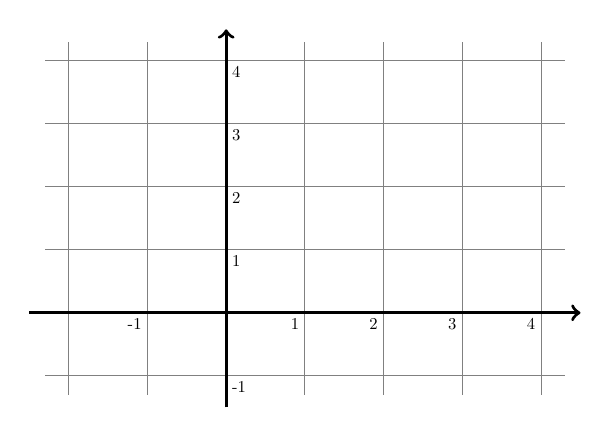
\begin{tikzpicture}[xscale=1,yscale=0.8]
\draw[gray] (-2.3,-1.3) grid (4.3,4.3);
\draw[very thick,->] (-2.5,0) -- (4.5,0);
\draw[very thick,->] (0,-1.5) -- (0,4.5);
\draw[very thick,color=blue] plot[domain=-1.3:3.3,samples=100] function {4-(x-1)**2};
\foreach \x in {1,...,4, -1} {
    \draw (\x, 0) node[below left, scale=0.6] {\x};
    \draw (0, \x) node[below right, scale=0.6] {\x};
}
\end{tikzpicture}
\end{flushright}
~\\
\end{minipage}
\hrule

%\question Simplify the following as much as possible. $\ds \frac{~\dfrac{1}{x+h} - \dfrac{1}{x}~}{h}$.
\vfill
%\hrule

\end{questions}
\end{document}
